% % % % % % % % % % % % % % % % % % % % % % % % % % % % % % % % % % % % % % % % % % % %
%                                                                                     %
% Short Sectioned Assignment LaTeX Template Version 1.0 (5/5/12)                      %
% This template has been downloaded from: http://www.LaTeXTemplates.com               %
%                                                                                     %
% Original author:  Frits Wenneker (http://www.howtotex.com)                          %
%                                                                                     %
% Modified by: Fco Javier Sueza Rodríguez (fcosueza@disroot.org)                      %
%                                                                                     %
% Changes:                                                                            %
%           - Document type scrarticle                                                %
%           - Use babel-lang-spanish package and marvosym                             %
%           - Use hyperref, enumitem and tcolorbox                                    %
%           - Use fancyhdr package an configure it                                    %
%           - Use Time New Roman (mathptmx), Helvetic and Courier fonts               %
%                                                                                     %
% License: CC BY-NC-SA 3.0 (http://creativecommons.org/licenses/by-nc-sa/3.0/)        %
%                                                                                     %
% % % % % % % % % % % % % % % % % % % % % % % % % % % % % % % % % % % % % % % % % % % %

%-----------------------------------------------%
%	              Packages                  %
%-----------------------------------------------%

\documentclass[bibliography=totoc]{scrarticle}

% ---- Text Input/Output ----- %

\usepackage[T1]{fontenc}
\usepackage[utf8]{inputenc}
\usepackage{mathptmx}
\usepackage[scaled=.92]{helvet}
\usepackage{courier}
\usepackage[indent=12pt]{parskip}
\usepackage[titletoc, title]{appendix}

\usepackage{geometry}
\geometry{verbose,tmargin=3cm,bmargin=3cm,lmargin=2.5cm,rmargin=2.5cm}

% ---- Language ----- %

\usepackage[spanish, es-tabla, es-noquoting]{babel}
\usepackage{marvosym}

% ---- Another packages ---- %

\usepackage[toc, sort=use]{glossaries}
\usepackage{amsmath,amsfonts,amsthm}
\usepackage{graphics,graphicx}
\usepackage{tcolorbox}
\usepackage{hyperref}
\usepackage{enumitem}
\usepackage{fancyhdr}
\usepackage{float}
\usepackage{ulem}


%--------------------------------------------------------------------%
%                      Customizing Document                          %
%--------------------------------------------------------------------%

% -------------- Customize headers and footers---------------------- %

\pagestyle{fancy}

\fancyhead[]{}
\fancyfoot[L]{}
\fancyfoot[C]{}
\fancyfoot[R]{\thepage}

\renewcommand{\headrulewidth}{0pt} % Remove header underlines
\renewcommand{\footrulewidth}{0pt} % Remove footer underlines

% Needed to get first page footer correctly
\fancypagestyle{plain}{
    \fancyhf{}
    \fancyfoot[R]{\thepage}
}

% --------------------- Packages Configuration --------------------- %


\hypersetup{
    colorlinks=true,
    linkcolor=magenta,
    urlcolor=magenta
}

\setcounter{secnumdepth}{4}
\setcounter{tocdepth}{4}
\graphicspath{{./images/}}

\setlength{\headheight}{13.6pt} % Customize the height of the header
\numberwithin{figure}{section} % Number figures within sections
\numberwithin{table}{section}

% ------------------------ New Commands ----------------------------- %

\newcommand{\horrule}[1]{\rule{\linewidth}{#1}} % Create horizontal rule command

% ------------------------ Anexx now with name in spanish before title ----------------------- %

\addto\captionsspanish{%
	\renewcommand\appendixname{Anexo}
	\renewcommand\appendixpagename{Anexos}
}




%----------------------------------------------------------------------------------------
%	TÍTULO Y DATOS DEL ALUMNO
%----------------------------------------------------------------------------------------

\title{
\vspace{10ex}
\normalfont \normalsize
\huge \textbf{Introducción a Apache Hadoop}
}
\author{Francisco Javier Sueza Rodríguez}
\date{\normalsize\today}

\glsenablehyper
\makeglossaries
\loadglsentries{glos}

%----------------------------------------------------------------------------------------
%                                     DOCUMENTO
%----------------------------------------------------------------------------------------
\begin{document}


\maketitle

\thispagestyle{empty}

\vspace{75ex}

\begin{center}
    \begin{tabular}{l l}
        \textbf{Centro}: & IES Zaidin-Vergeles \\
        \textbf{Curso}: & Inteligencia Artificial y Big Data\\
        \textbf{Módulo}: & Big Data Aplicado \\
    \end{tabular}
\end{center}

\newpage

\begingroup
\hypersetup{linkcolor=black}
\tableofcontents
\endgroup

\newpage

\begingroup
\hypersetup{linkcolor=black}
\listoffigures             
\endgroup

\newpage

\section{Creación de la Máquina Virtual}
Crea en Oracle VirtualBox una máquina virtual con Ubuntu Server 26.04 LTS, 2 procesadores virtuales, 8 GB de RAM, 100 GB de almacenamiento y una configuración de red que permita acceso a Internet y a las interfaces web de Hadoop desde el equipo anfitrión.

\subsection{Solución}
En este primer ejercicio se va a proceder a instalar \textbf{Ubunut Server 26.04.1} en una máquina virtual de \textbf{VirtualBox}, la cual se ha instalado en el sistema operativo del host, que es una \textbf{Kubuntu 26.04.1}, y se ha creado una imagen usando es especificaciones indicadas.

En primer lugar se ha creado la imagen con el nombre \textbf{practica1-bda}, esto no estaba especificado en la practica por lo que se ha elegido este para dejar claro su propósito. La imagen se ha creado casi de forma automática, solo especificando algunos datos durante el proceso.

Se ha creado el \textbf{usuario hadoop}, tal y como se especificaba en el enunciado, pero la ir a crear le \textbf{hostname} con las indicaciones dadas ha surgido un problema, y es que Linux \textbf{no admite la barra baja} (\_) como carácter para nombrar el hostname, por lo que sea ha sustituido por la barra media. Eso se debe a que según el estándar \cite{rfc01}, no se puede emplear este carácter para el hostname.

En la siguiente captura se puede ver la configuración general generada después de crear la imagen:

\begin{figure}[ht]
	\centering
	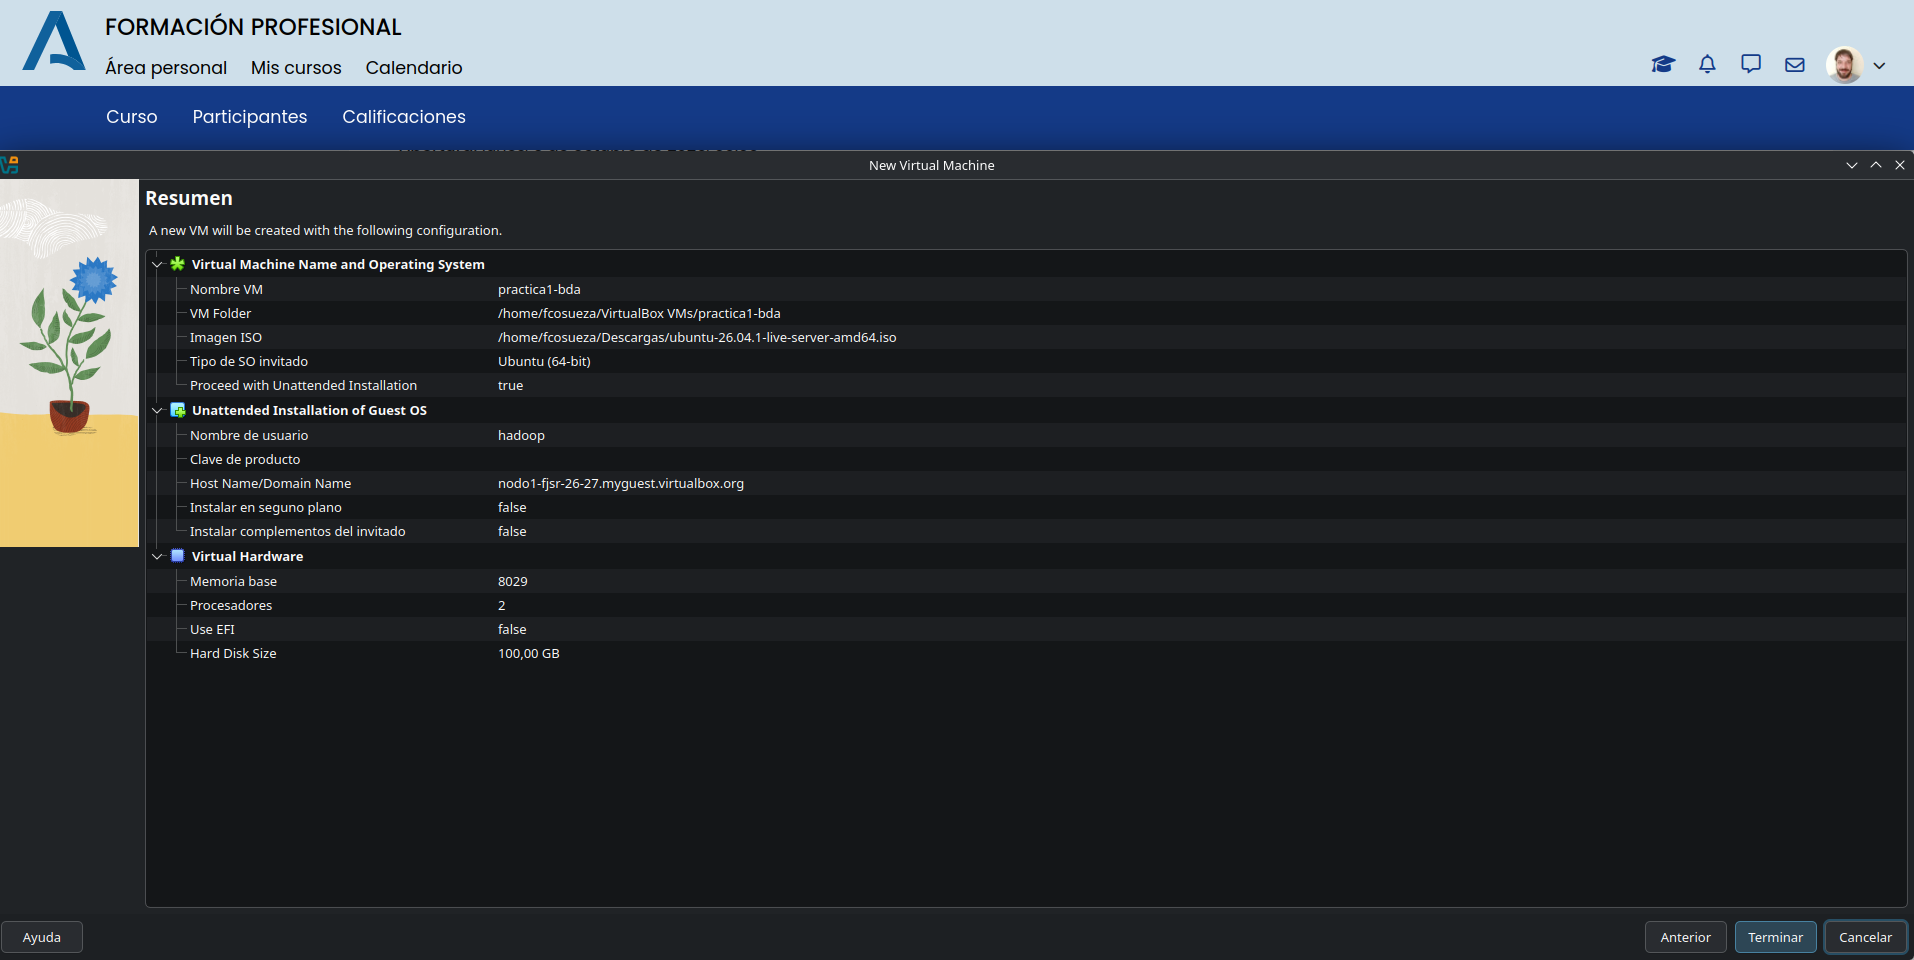
\includegraphics[scale=0.32]{virtual-config-gen.png}
	\caption{Configuración General de la Imagen}
\end{figure}
	
Después de realizar la configuración general, se ha elegido el \textbf{número de CPUs} que queremos que tenga la imagen, que este caos han sido 2, y la \textbf{cantidad de RAM} que va a tener la máquina virtual, que va a ser un total de \textbf{8 GB}, tal y como se especifica en el enunciado.

En la siguiente captura, tomada durante el proceso de creación, se puede ver esta información:

\begin{figure}[H]
	\centering
	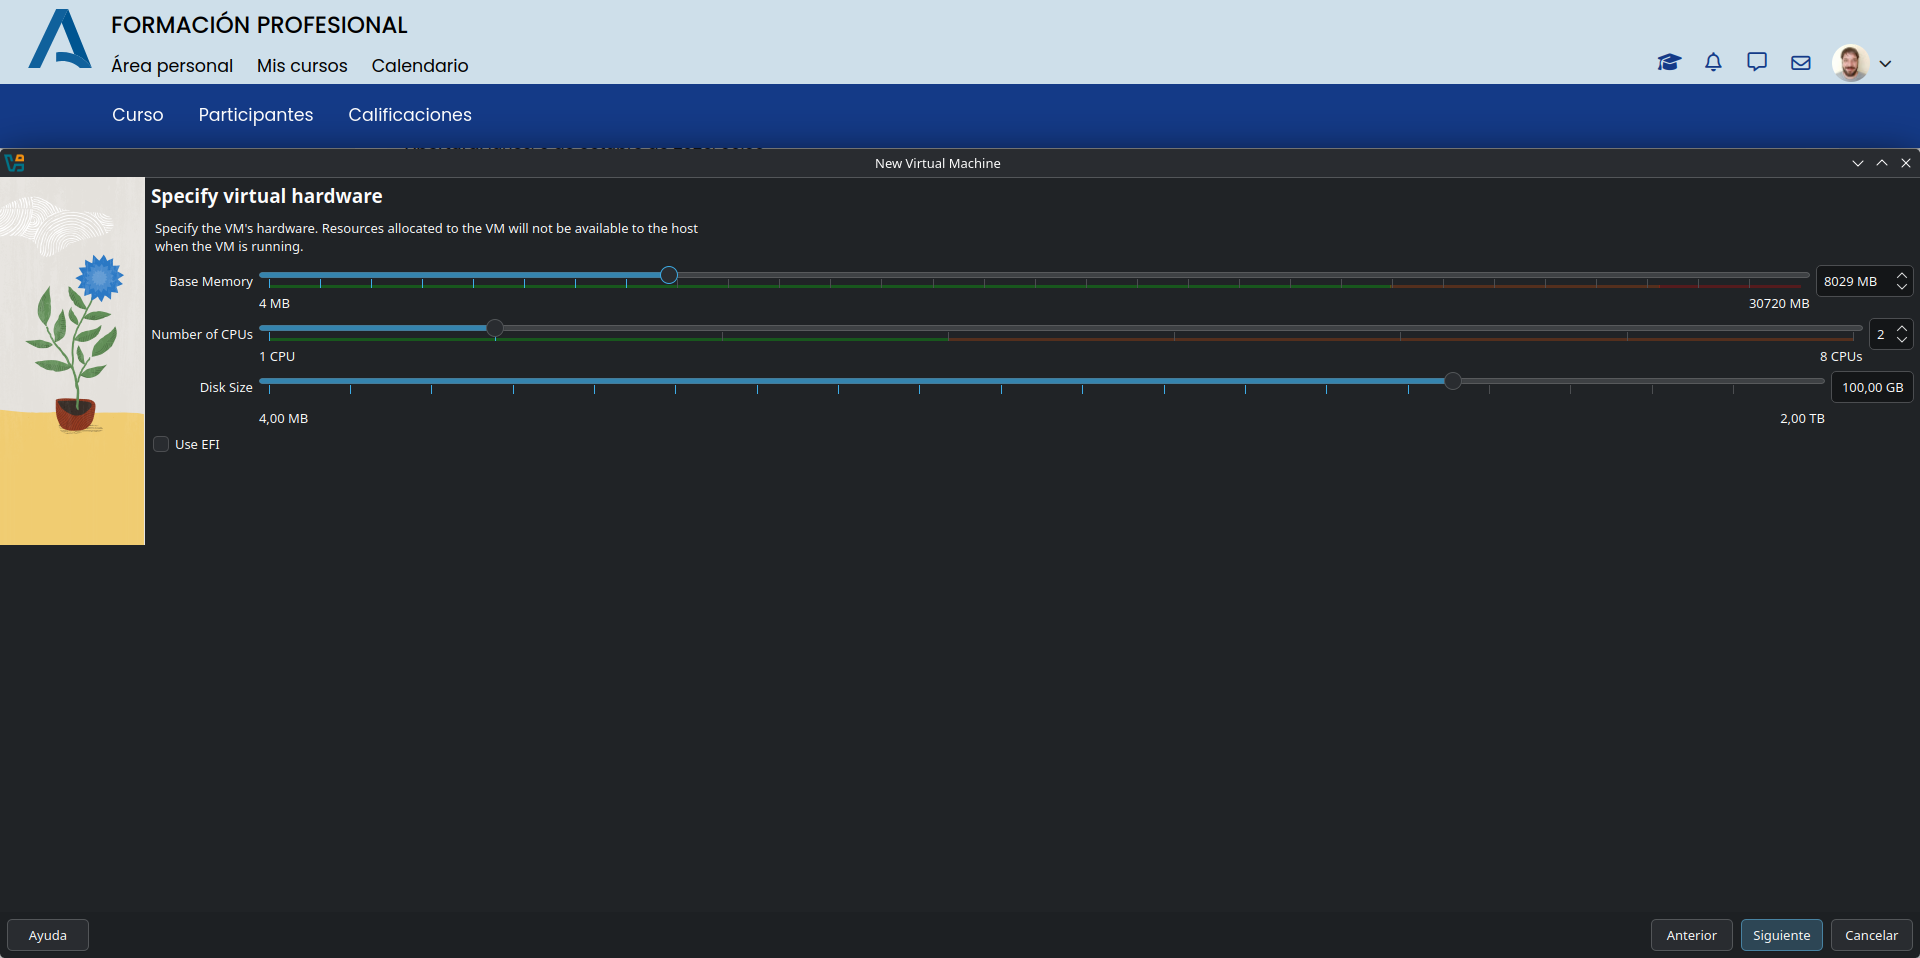
\includegraphics[scale=0.32]{virtual-config-cpu.png}
	\caption{Configuración de CPU/RAM de la Imagen}
\end{figure}

También se ha seleccionado \textbf{100 GB de almacenamiento}, como podemos ver en la primera captura. El resto de la configuración se ha creado de forma automática, durante el proceso de creación de la imagen, como por ejemplo, el adaptador de red que se usa. En la siguiente captura, podemos ver la configuración creada tanto del Almacenamiento como de red:

\begin{figure}[ht]
	\centering
	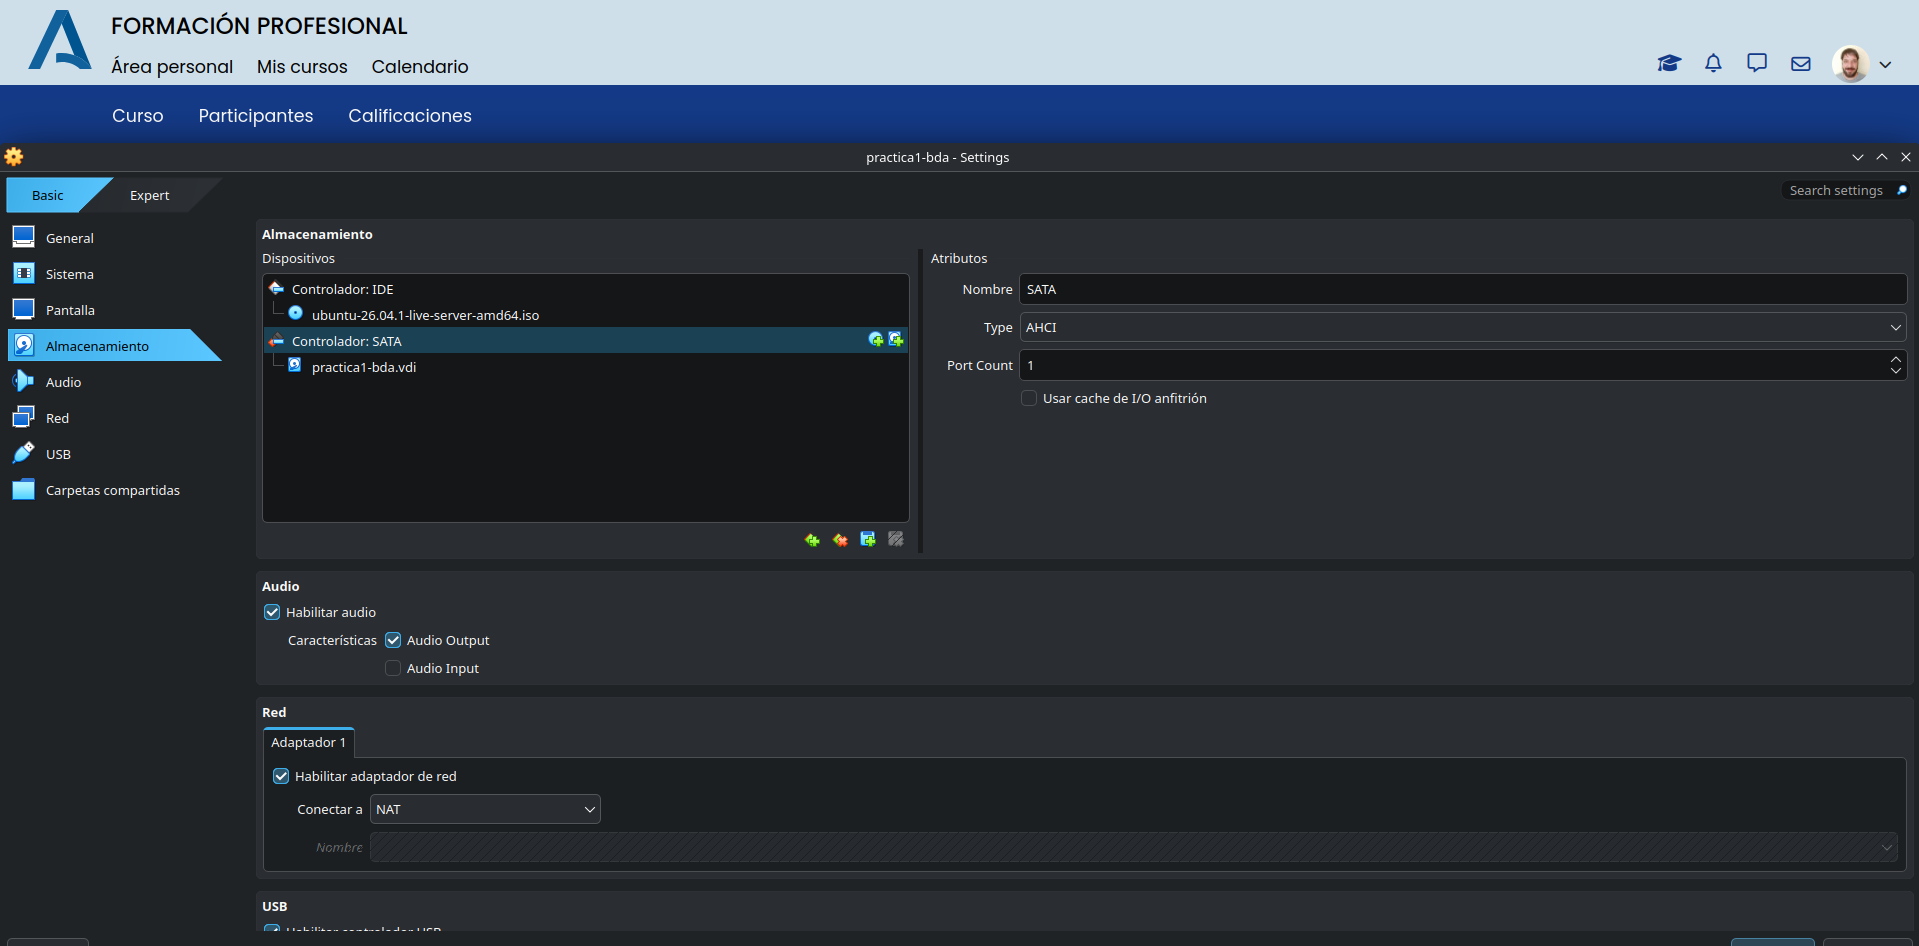
\includegraphics[scale=0.32]{virtual-config-red.png}
	\caption{Configuración del Alamacenamiento y de Red de la Imagen}
\end{figure}

Como podemos ver, ha configuración la conexión de red automáticamente con \textbf{NAT}, así como el controlador SATA para el almacenamiento.

Una vez realizada la configuración, se ha \textbf{instalado Ubuntu Server} en la máquina virtual. Una vez realizada la instalación, se ha \textbf{iniciado Ubuntu Server} por primera, como podemos ver a continuación:

\begin{figure}[ht]
	\centering
	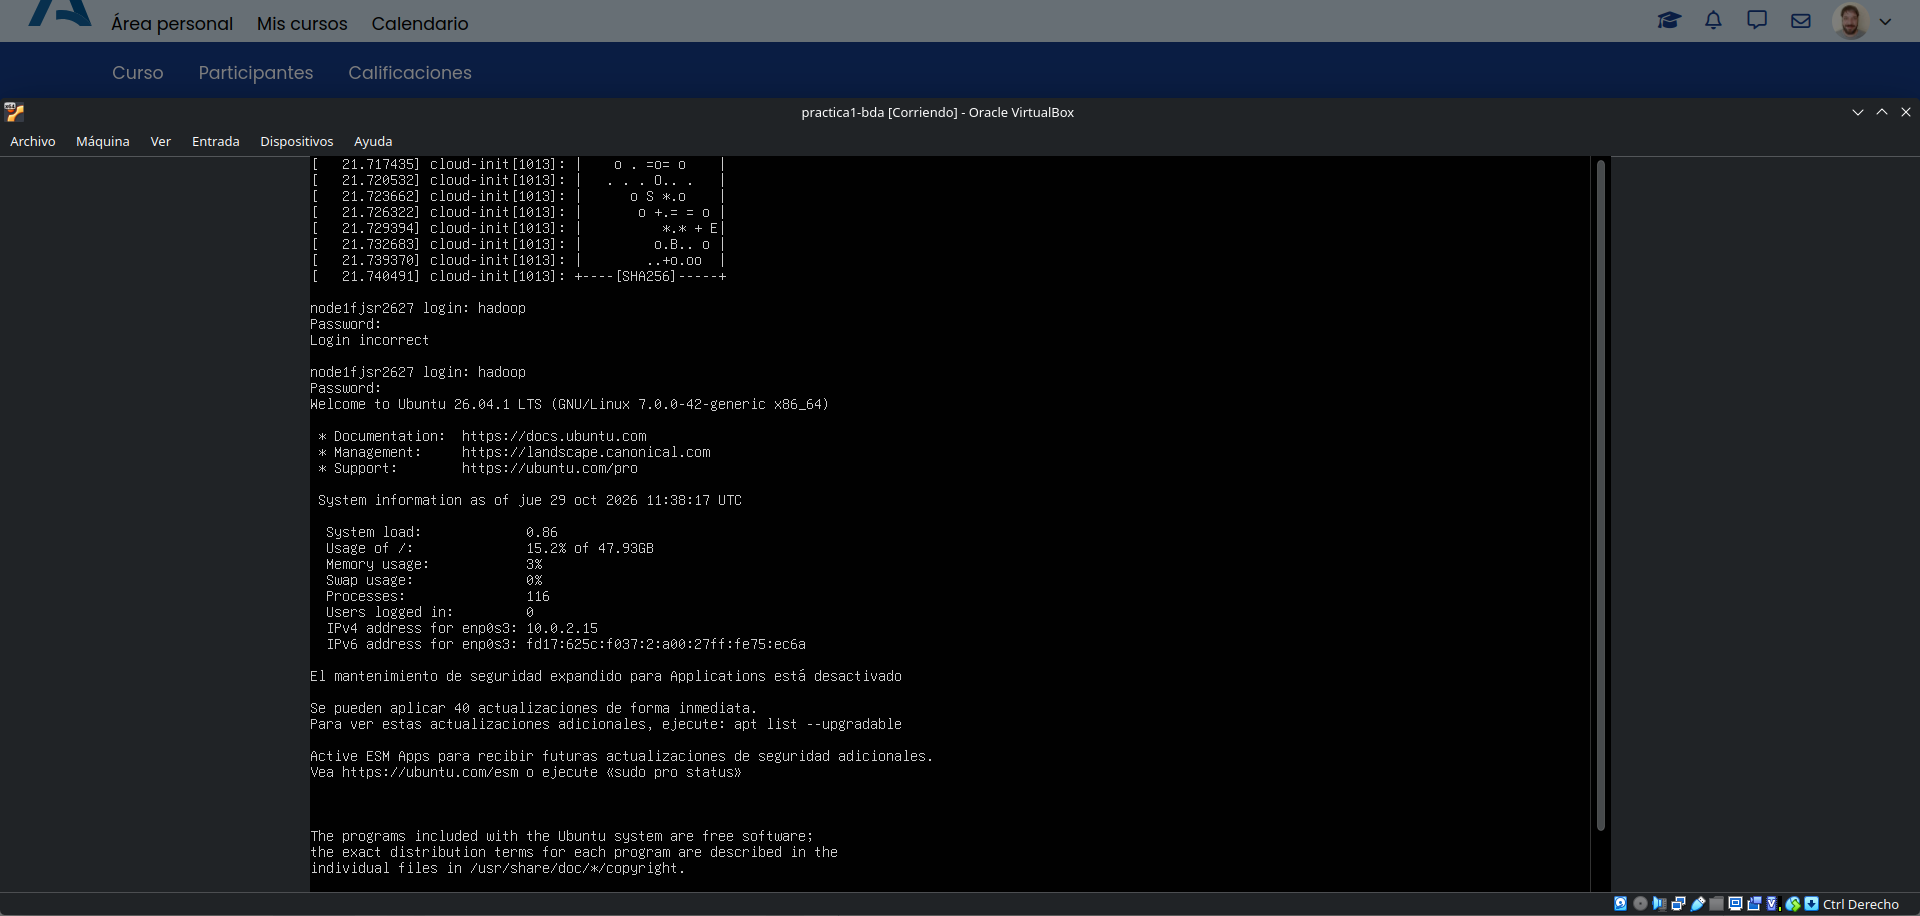
\includegraphics[scale=0.32]{virtual-config-init.png}
	\caption{Primer inicio de Ubuntu Server}
\end{figure}

\section{Configuración del Nombre del Equipo y Preparación del Sistemas}
Configura el nombre del nodo con el formato \textbf{nodo1\_iniciales\_26\_27}, compruébalo con \textbf{hostname} y \textbf{hostnamectl}, actualiza el sistema, verifica la conectividad e instala Java. Explica por qué Hadoop necesita Java y la función de \textbf{JAVA\_HOME}.

\subsection{Solución}
Como se comentaba en el punto anterior, \textbf{ni Linux}, \textbf{ni VirtualBox permiten} los nombres de host con \textbf{guiones bajos}, así que se ha optado por reemplazar los guiones bajos por guiones medios, para evitar conflictos. En la siguiente captura, podemos ver la ejecución de los comandos \textbf{hostname} y \textbf{hostnamectl}.

\begin{figure}[ht]
	\centering
	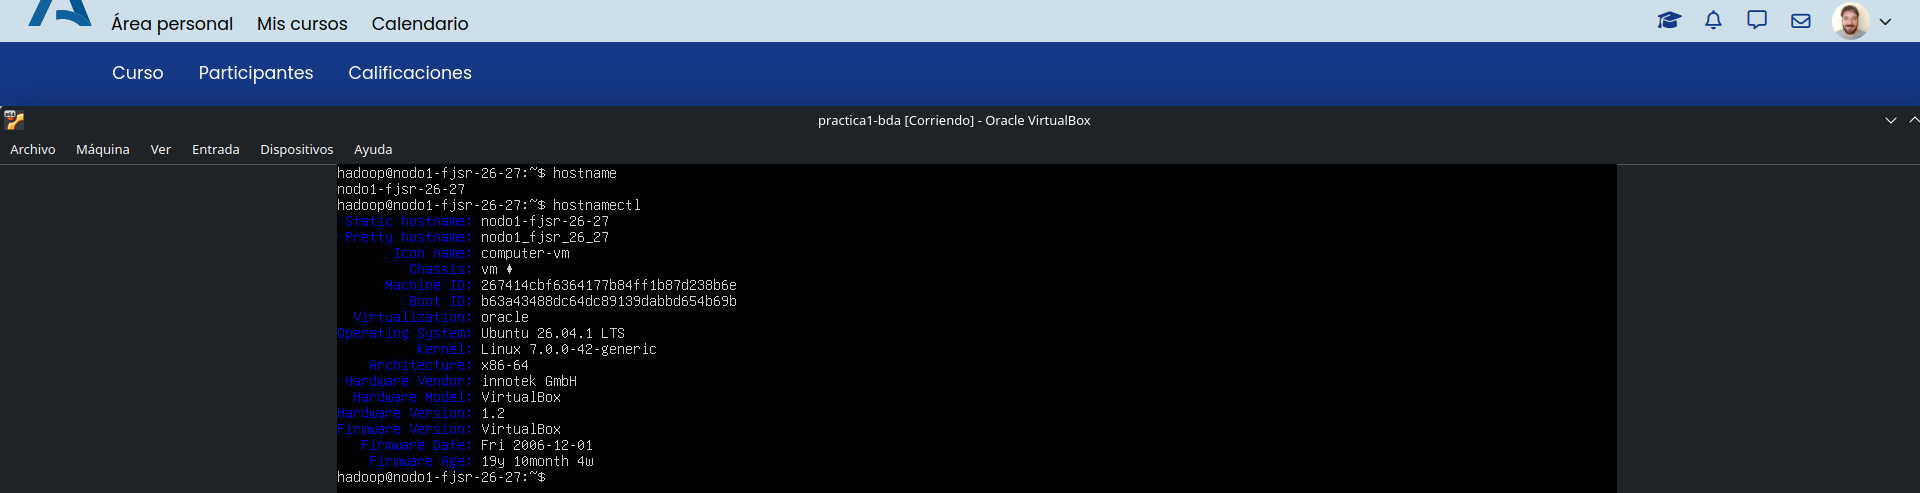
\includegraphics[scale=0.32]{hostname.png}
	\caption{Ejecución de los comandos hostname y hostnamectl}
\end{figure}

A continuación se ha actualizado el sistemas, empleando el comando \textbf{sudo apt-get update} y se ha procedido a instalar Java, mediante los paquetes \textbf{default-jre} y \textbf{default-jdk}, que se han instalado sin problemas. En la siguiente captura, podemos ver la versión instalada de Java:

\begin{figure}[ht]
	\centering
	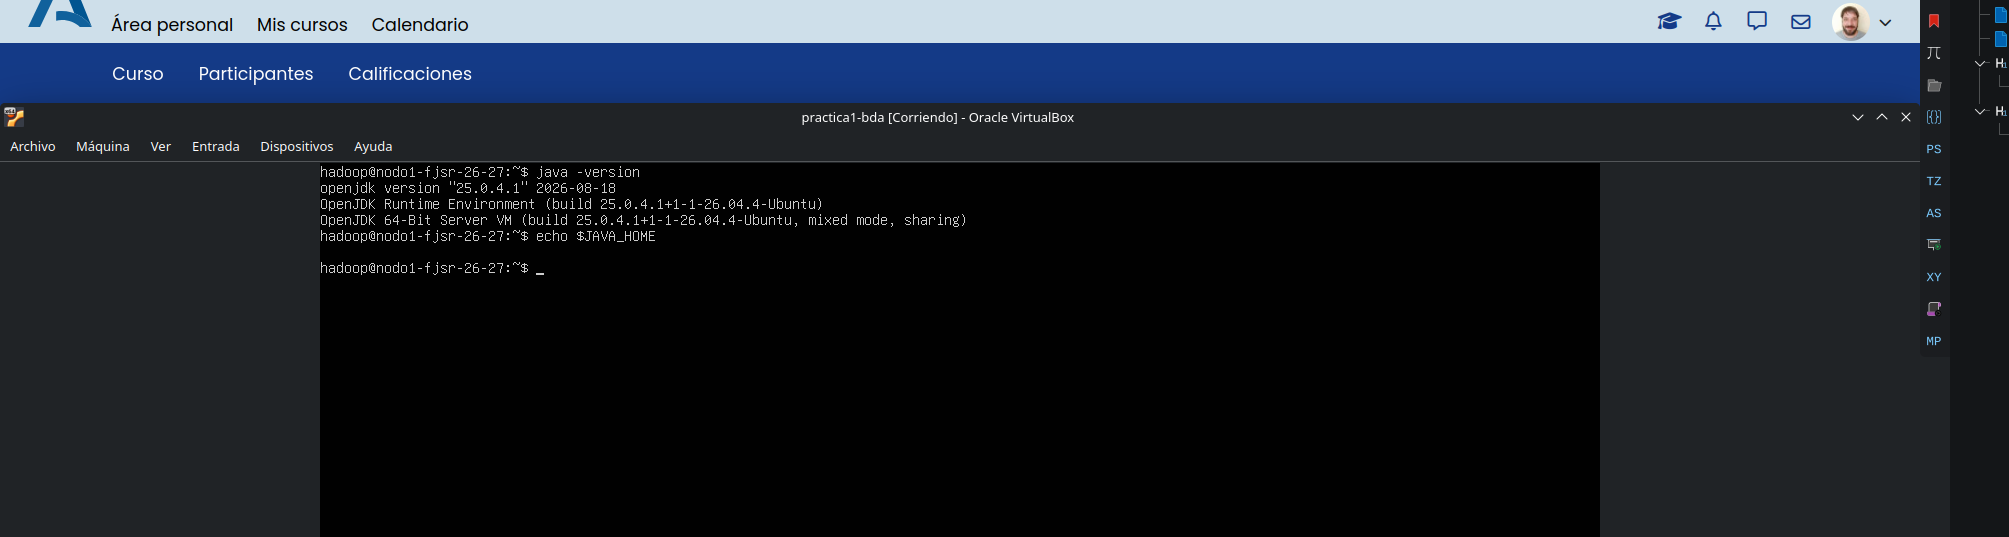
\includegraphics[scale=0.32]{java-install.png}
	\caption{Versión de Java instalada}
\end{figure}

El motivo por que Hadoop es porque \textbf{esta desarrollado en Java}, especialmente las librerías principales del proyecto, aunque hay otros lenguajes que se incluyen en otras aplicaciones del ecosistemade Hadoop \cite{ibm01}. Respecto a \textbf{JAVA\_HOME}, es una variable de entorno importante, ya que apunta al \textbf{entorno de ejecución de JAVA}, o \textbf{JRE} (Java Runtime Environment).

\section{Creación del Usuario Hadoop}
Crea el usuario \textbf{hadoop}, su directorio personal, configura los permisos necesarios y accede con dicho usuario. El prompt debe tener un formato similar a \textbf{hadoop@nodo1\_abs\_26\_27:~\$}.

\subsection{Solución}
El usuario hadoop \textbf{se ha creado} durante el proceso de \textbf{instalación}, por lo que no ha sido necesario crearlo ahora, aunque hubiera sido sencillo usando el comando \textbf{adduser}, pero no ha sido necesario. En la siguiente captura se puede ver el prompt correcto.

\begin{figure}[ht]
	\centering
	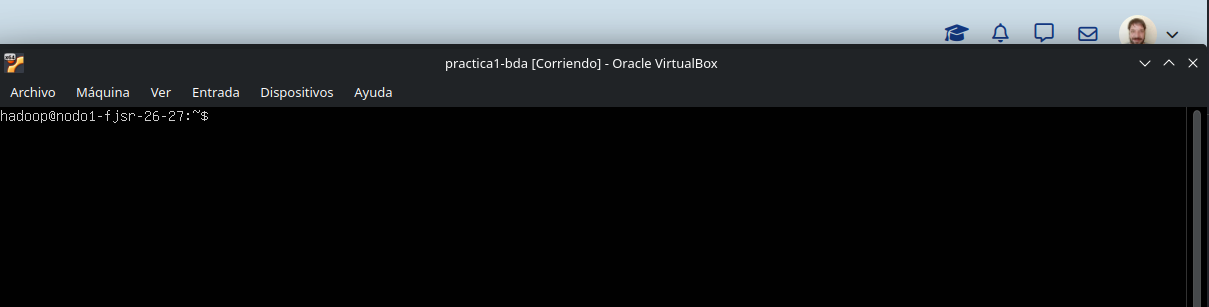
\includegraphics[scale=0.50]{user.png}
	\caption{Prompt con el usuario y el hostname}
\end{figure}

\section{Configuración de SSH}
Instala y configura SSH para que el usuario \textbf{hadoop} pueda conectarse sin contraseña mediante clave pública. Prueba \textbf{ssh localhost} y \textbf{ssh nodo1\_iniciales\_26\_27}. Explica por qué Hadoop utiliza SSH.

\subsection{Solución}












\newpage

\bibliography{citas}
\bibliographystyle{unsrt}


\end{document}  